% =====================================================================
%  The discrete <-> continuous bridge for the Riemann zeta / Dirichlet
%  eta functions: a zero-birth knob, a midpoint warp onto zeta(s,1/2),
%  and a unified O(1/K) rate law.
%
%  A computational / experimental-mathematics preprint.
%  Build:  tectonic main.tex      (see README.md in this directory)
% =====================================================================
\documentclass[11pt]{article}

\usepackage[a4paper,margin=1in]{geometry}
\usepackage[T1]{fontenc}
\usepackage[utf8]{inputenc}
\usepackage{lmodern}
\usepackage{microtype}

\usepackage{amsmath,amssymb,amsthm,mathtools}
\usepackage{graphicx}
\usepackage{booktabs}
\usepackage{tabularx}
\usepackage{enumitem}
\usepackage{xcolor}

\usepackage[numbers,sort&compress]{natbib}
\usepackage[colorlinks=true,linkcolor=blue!55!black,citecolor=blue!55!black,urlcolor=blue!55!black]{hyperref}
\usepackage[capitalise,nameinlink]{cleveref}

% Figures live in the canonical drivers' output dir; a local copy under
% figures/ (made by the arXiv packaging step) takes precedence.
\graphicspath{{figures/}{../bridge/figures/}}

% ---- light theorem-like environments (no theorems are claimed) -------
\theoremstyle{definition}
\newtheorem{observation}{Observation}
\newtheorem{remark}{Remark}

% ---- notation -------------------------------------------------------
\renewcommand{\Re}{\operatorname{Re}}
\renewcommand{\Im}{\operatorname{Im}}
\newcommand{\dd}{\mathrm{d}}
\newcommand{\eu}{\mathrm{e}}
\newcommand{\half}{\tfrac12}

\title{\bfseries A discrete\,$\leftrightarrow$\,continuous bridge for the
Riemann zeta and Dirichlet eta functions:\\
a zero-birth knob, a midpoint warp onto $\zeta(s,\tfrac12)$,\\
and a unified $O(1/K)$ rate law}

\author{Brad Martin\thanks{\texttt{1bradley.martin1@gmail.com}. Source code
and reproduction scripts: \url{https://github.com/bradleypmartin/dirichlet-bridge}.}}

\date{\today}

\begin{document}
\maketitle

\begin{abstract}
We study a one-parameter family of analytic objects that interpolates from the
bland continuous integral $\int_1^\infty x^{-s}\,\dd x = 1/(s-1)$ (which keeps
$\zeta$'s pole but has \emph{no} non-trivial zeros, no functional equation, and no
arithmetic) to the full Dirichlet series $\zeta(s)$. The interpolation knob is
the number $K$ of Fourier harmonics of the discreteness kernel (the
Euler--Maclaurin sawtooth, equivalently the Abel--Plana comb) that one retains.
As $K$ grows, the non-trivial zeros are \emph{born} out of a literally zeroless
endpoint and then \emph{migrate} onto their critical lines. We exhibit two
routes to the same destination, an \emph{additive} comb that adds harmonics to
the integrand and a \emph{nonlinear midpoint warp} of the integration variable
that is deliberately engineered to land on the half-shifted Hurwitz zeta
$\zeta(s,\tfrac12) = (2^s-1)\zeta(s)$; and we record the general-phase warp
onto $\zeta(s,\alpha)$, which reproduces the Saias--Weingartner $P\cdot L$
dichotomy (clean vertical zero strings only at $\alpha\in\{0,\tfrac12,1\}$). The
unifying result is a single \emph{$O(1/K)$ rate / birth-$K$ law}: every route
truncates the same sawtooth, so every route converges at the same algebraic rate,
with a route-dependent displacement constant whose real part fixes the approach
side and whose imaginary part is numerically tied to Gram's law. Finally we read
the Dirichlet-$\eta$ zeros as a two-component ``crystal $\times$ GUE'' spectrum
and isolate the single prime $p=2$. This is a \emph{computational /
experimental-mathematics} synthesis: every individual endpoint is classical and
is cited as such; the contribution is the unifying construction, the rate law,
and the spectral readings, not a new theorem about where zeros live. All figures
and numbers are reproducible from the accompanying repository.
\end{abstract}

\tableofcontents

% =====================================================================
\section{Introduction}\label{sec:intro}
% =====================================================================

The Riemann zeta function $\zeta(s) = \sum_{n\ge 1} n^{-s}$ is a \emph{discrete}
object: a sum over the integers. Its simplest continuous shadow is the integral
that replaces the sum by its leading Euler--Maclaurin term,
\begin{equation}\label{eq:bland}
  \int_1^\infty x^{-s}\,\dd x = \frac{1}{s-1}, \qquad \Re s > 1,
\end{equation}
which retains $\zeta$'s pole at $s=1$ but is otherwise inert: it has \emph{no}
non-trivial zeros, no functional equation, and no arithmetic content whatsoever.
The gap between \eqref{eq:bland} and the genuine $\zeta(s)$ is the
discreteness of the integers, and the Euler--Maclaurin formula makes that gap
explicit as a sum of correction terms built from the periodic Bernoulli
``sawtooth'' $\widetilde B_1(x) = \{x\}-\tfrac12$. The Fourier series of the
sawtooth,
\begin{equation}\label{eq:sawtooth}
  \widetilde B_1(x) = \{x\}-\tfrac12 = -\sum_{k\ge 1}\frac{\sin(2\pi k x)}{\pi k},
\end{equation}
suggests an obvious interpolation knob: keep only the first $K$ harmonics. At
$K=0$ one is back at the bland endpoint \eqref{eq:bland}; as $K\to\infty$ one
restores the full discreteness and recovers $\zeta(s)$.

This paper studies what the non-trivial zeros do along that interpolation. The
short answer, made literal and visual throughout, is that the zeros are
\emph{born} as $K$ leaves $0$ and then \emph{migrate} onto their critical lines as
$K\to\infty$. Because the $K=0$ endpoint is genuinely zeroless, this is a
\emph{creation-and-migration} mechanism, not a rearrangement of a pre-existing
zero set; we contrast it carefully with the de Bruijn--Newman heat flow in
\cref{sec:prior}.

\paragraph{Honest framing.}
We state at the outset, as a deliberate decision, that this is a \emph{methods /
experimental-mathematics} paper: a unified, reproducible re-derivation that
threads several \emph{known} endpoints onto one explicit ``restore discreteness''
knob and measures how the zeros respond. It is \emph{not} a theorem about where
the zeros of $\zeta$ live, and it carries no implication toward the Riemann
hypothesis. Every individual ingredient below is classical, and we have made two
adversarial passes through the literature to keep the attribution honest. What is
classical, and what we believe is the surviving synthesis, is stated plainly here
and revisited in \cref{sec:prior}:

\begin{itemize}[leftmargin=1.4em]
\item \textbf{Classical (we cite, we do not claim):} the half-shift identity
  $(2^s-1)\zeta(s)=\zeta(s,\tfrac12)$ and the migration of Hurwitz-type zeros
  onto $\sigma=\tfrac12$ \citep{Gonek1981,GarunkstisSteuding2007}; the privileged
  $\alpha\in\{0,\tfrac12,1\}$ $P\cdot L$ dichotomy
  \citep{SaiasWeingartner2009}, with generic off-line $\zeta(s,\alpha)$ zeros
  \citep{DavenportHeilbronn1936,Cassels1961}; the $\sigma=1$ eta comb at
  $t=2\pi k/\ln 2$ \citep{Sondow2003,BeliakovMatiyasevich2015}; and the
  appearance of prime-power log-frequencies (smallest $\ln 2$) in the
  zeta-zero number variance, in a regime where the GUE prediction fails
  \citep{Berry1988,LugarMilinovichQuesadaHerrera2022}.
\item \textbf{The synthesis we offer:} the harmonic-count $K$ as a
  \emph{zero-birth knob} attached to a literally zeroless endpoint; the
  Euler--Maclaurin sawtooth $\equiv$ Abel--Plana comb identity read as a
  zero-birth event; the midpoint warp \emph{deliberately} landing on
  $\zeta(s,\tfrac12)$ (with its $\sigma=0$ companion as the functional-equation
  mirror of $\eta$'s $\sigma=1$ comb); a \emph{unified $O(1/K)$ rate law} tying
  the additive and warp routes together, with a Gram's-law coupling on the
  vertical axis; and a comb\,$\uplus$\,GUE two-component reading of the $\eta$
  zeros that isolates the single prime $p=2$.
\end{itemize}

\paragraph{Roadmap.}
\Cref{sec:endpoints} sets up the two endpoints: the bland $1/(s-1)$ and the
structured continuous-$\eta$ integral, whose off-critical zero string already
obeys the Riemann--von Mangoldt counting law. \Cref{sec:comb} restores
discreteness \emph{additively} and exhibits the zero-migration map.
\Cref{sec:warp} restores it by a nonlinear \emph{warp} of the integration
variable, deliberately targeting $\zeta(s,\tfrac12)$, and leads with the algebra
that makes the half-integer object \emph{contain} $\zeta$. \Cref{sec:alpha}
generalizes the warp to arbitrary phase and recovers the $P\cdot L$ dichotomy.
\Cref{sec:rate} is the unifying $O(1/K)$ rate law. \Cref{sec:two} reads the
$\eta$ zeros as a two-component spectrum. \Cref{sec:prior} foregrounds the
prior-art deflators and gives the de Bruijn--Newman contrast, and
\cref{sec:repro} points to the reproducible code.

% =====================================================================
\section{The two endpoints}\label{sec:endpoints}
% =====================================================================

\subsection{The bland endpoint}
For $\Re s>1$, \eqref{eq:bland} is the entire continuous content of the leading
Euler--Maclaurin term applied to $\zeta$. Analytically continued, $1/(s-1)$ is a
meromorphic function with a single simple pole and \emph{no zeros at all}. It is
the honest ``$K=0$'' object on the $\zeta$ side: pole present, everything else
absent.

\subsection{The structured continuous endpoint}
The alternating (Dirichlet) eta function $\eta(s) = \sum_{n\ge 1}(-1)^{n-1}
n^{-s} = (1-2^{1-s})\zeta(s)$ has a more interesting continuous shadow, because
the alternating sign is $(-1)^n = \cos(\pi n)$ at the integers. Replacing the sum
by the corresponding integral gives
\begin{equation}\label{eq:conteta}
  F(s) \;=\; \int_1^\infty \cos(\pi x)\, x^{-s}\,\dd x,
\end{equation}
which, unlike \eqref{eq:bland}, is genuinely structured: it has a closed form in
incomplete gamma functions and a non-trivial zero string. Numerically (see
\cref{fig:conteta}) the zeros of \eqref{eq:conteta} obey three laws, confirmed to
$3$--$5$ digits over $8<t<160$:
\begin{align}
  \text{(real part)} &\quad \sigma(t)\to \tfrac32, \label{eq:re32}\\
  \text{(spacing)}   &\quad \Delta t \sim \frac{2\pi}{\ln(t/\pi)}, \label{eq:spacing}\\
  \text{(counting)}  &\quad N(t) = \frac{t}{2\pi}\ln\frac{t}{\pi \eu} + \frac58, \label{eq:rvm}
\end{align}
the last of which is the Riemann--von Mangoldt counting form familiar from $\zeta$
itself \citep{Riemann1859,Titchmarsh1986}.

\begin{figure}[t]
  \centering
  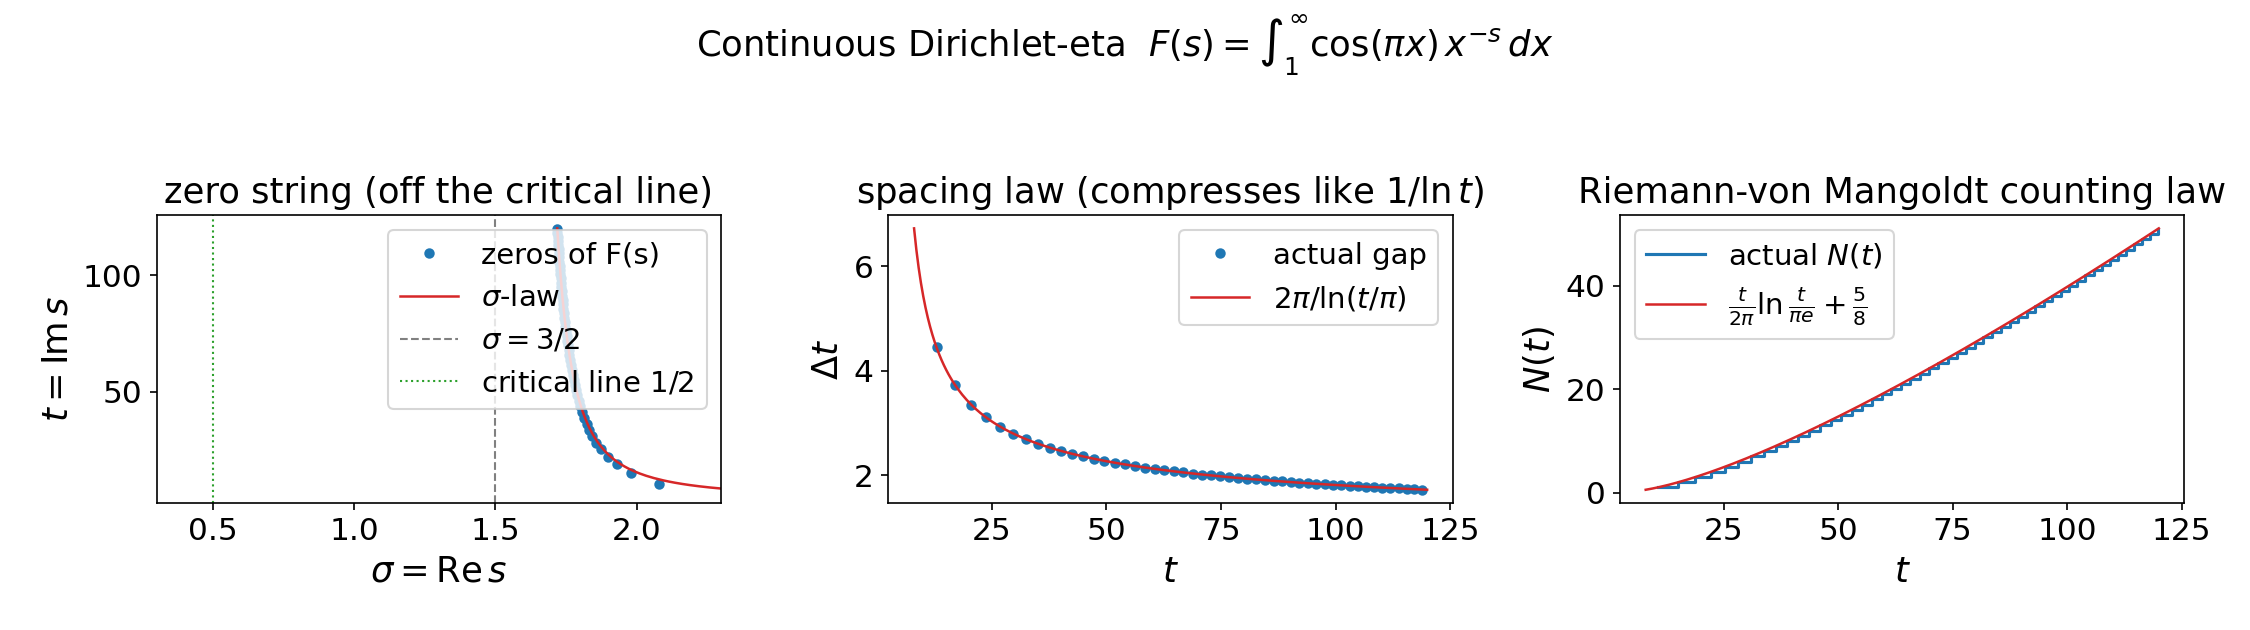
\includegraphics[width=0.92\textwidth]{cont_eta.png}
  \caption{The continuous-$\eta$ endpoint $F(s)=\int_1^\infty\cos(\pi
  x)x^{-s}\dd x$ and its off-critical zero string. The zeros have the
  \emph{right density} (the Riemann--von Mangoldt law \eqref{eq:rvm}), but
  their real parts drift toward $\sigma=\tfrac32$ \eqref{eq:re32}: the continuum
  supplies ``non-trivial zeros with the correct counting law'' but not ``zeros on
  the critical line.''}
  \label{fig:conteta}
\end{figure}

\begin{observation}\label{obs:density}
The continuous endpoint already supplies non-trivial zeros with the
\emph{correct Riemann--von Mangoldt density} \eqref{eq:rvm}; what it withholds is
their \emph{location}. The zeros live off the critical line, drifting toward
$\sigma=\tfrac32$. ``Zeros with the right counting law'' is therefore a property
of the continuum; ``those zeros on $\Re s = \tfrac12$'' is what restoring
discreteness must supply. Closing that gap is the whole point of the bridge.
\end{observation}

% =====================================================================
\section{Phase 1: the additive comb}\label{sec:comb}
% =====================================================================

The first route restores discreteness \emph{additively}: add the Fourier
harmonics \eqref{eq:sawtooth} of the discreteness kernel back into the integrand,
one at a time, and track each zero as a curve in $K$. We call the resulting
trajectories the \emph{zero-migration map} (\cref{fig:comb}).

\paragraph{Two integral guises of one comb.}
The discreteness correction admits two classical integral representations that we
verify agree term by term: the Euler--Maclaurin sawtooth $\widetilde B_1(x) =
\{x\}-\tfrac12$ and the Abel--Plana ``Bose'' comb $1/(\eu^{2\pi x}-1)$. They are
the same object viewed through two windows; truncating either at $K$ harmonics
gives the identical interpolant. We read this shared truncation as the engine of
the rate law in \cref{sec:rate}.

\paragraph{Birth on the $\zeta$ side.}
On the $\zeta$ side the zeroless endpoint is $1/(s-1)+\tfrac12$ (the integral plus
the constant Euler--Maclaurin term). As the \emph{first} harmonic switches on, the
non-trivial zeros are literally \emph{born}, and they then slide onto
$\sigma=\tfrac12$ as $K$ increases. There is no zero to ``move'' at $K=0$; the
zero set is created.

\paragraph{Splitting on the $\eta$ side.}
On the $\eta$ side the $K=0$ ground string \emph{splits} as $K$ grows: half the
zeros onto $\sigma=\tfrac12$ (the genuine $\zeta$ zeros) and half onto $\sigma=1$
(the zeros of the prefactor $1-2^{1-s}$, located at $t=2\pi m/\ln 2$). This split
is a near-bijection of densities: writing the two pieces out,
\begin{equation}\label{eq:etadensity}
  \underbrace{\frac{t}{2\pi}\ln\frac{t}{2\pi \eu}}_{\sigma=1/2\ \text{(critical line)}}
  \;+\;
  \underbrace{\frac{t\ln 2}{2\pi}}_{\sigma=1\ \text{(prefactor comb)}}
  \;=\;
  \frac{t}{2\pi}\ln\frac{t}{\pi \eu},
\end{equation}
which recovers the continuous endpoint's density \eqref{eq:rvm}. No zeros are
created or destroyed in the $\eta$ migration; the existing string is \emph{sorted}
onto two lines, and the driver's counting check witnesses
\eqref{eq:etadensity} numerically.

\begin{figure}[t]
  \centering
  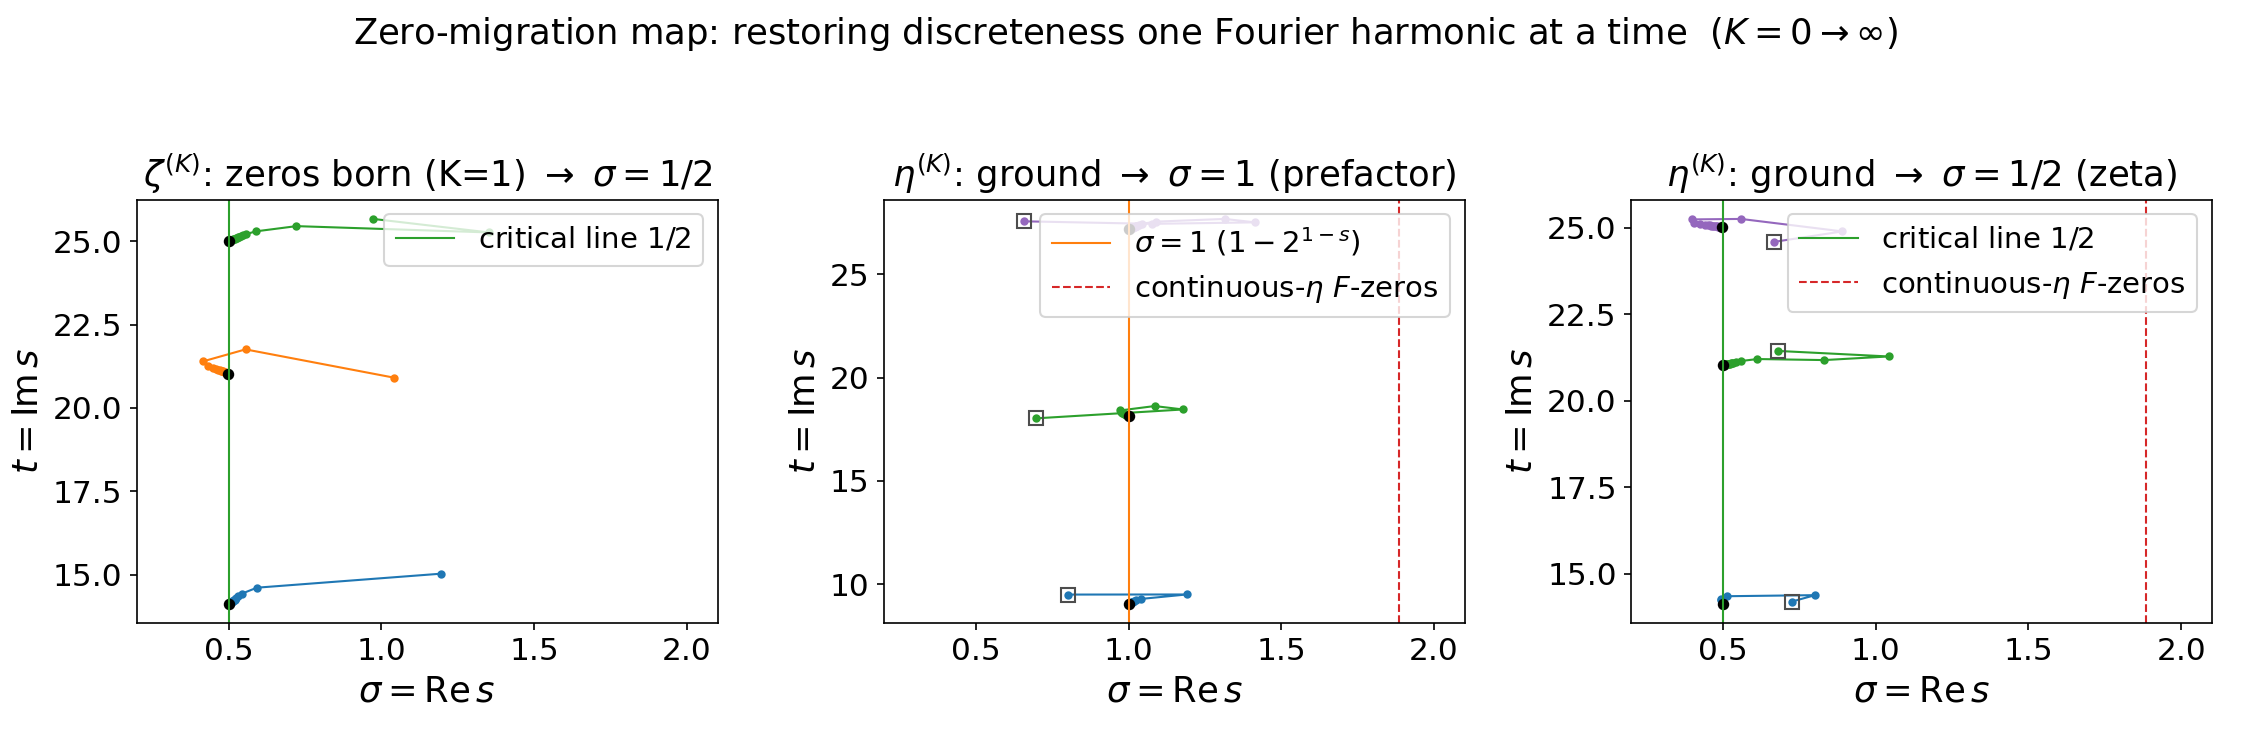
\includegraphics[width=0.92\textwidth]{harmonic_bridge.png}
  \caption{The additive zero-migration map: restoring discreteness one harmonic
  at a time. On the $\zeta$ side the zeros are \emph{born} as the first harmonic
  switches on and slide onto $\sigma=\tfrac12$; on the $\eta$ side the ground
  string \emph{splits} onto $\sigma=\tfrac12$ (the $\zeta$ zeros) and $\sigma=1$
  (the $1-2^{1-s}$ comb at $t=2\pi m/\ln 2$), conserving the density
  \eqref{eq:etadensity}.}
  \label{fig:comb}
\end{figure}

% =====================================================================
\section{Phase 2: the nonlinear midpoint warp}\label{sec:warp}
% =====================================================================

The second route reaches the critical line by a different mechanism: instead of
adding harmonics to the integrand, we \emph{warp the integration variable} so the
measure is pulled toward integer plateaus, $n^\ast = x + \varphi_K(x)$, where
$\varphi_K$ is the $K$-harmonic truncation of the sawtooth displacement. As
$K\to\infty$ the warp collapses each unit cell onto its \emph{midpoint}, so its
natural target is the half-shifted Hurwitz zeta. Before the figures, we state the
algebra that makes this target legitimate, which is the single most likely reader
sticking point.

\subsection{Why the half-integers reproduce $\zeta$'s own zeros}\label{sec:legit}

A fair worry: the literal Dirichlet series is summed over the counting numbers
$1,2,3,\dots$ (that is the $\alpha=1$ warp of \cref{sec:alpha}), so why should a
\emph{half-integer} object reproduce $\zeta$'s zeros and their migration at all?
Because the half-integer object is not a different beast that merely mimics
$\zeta$; it \emph{contains $\zeta$ as a factor}, by an exact identity. The
half-integers are the odd integers rescaled by $\tfrac12$:
\begin{equation}\label{eq:oddsum}
  \zeta(s,\tfrac12) = \sum_{n\ge 0}(n+\tfrac12)^{-s}
  = 2^{s}\sum_{n\ge 0}(2n+1)^{-s}
  = 2^{s}\!\!\sum_{m\ \mathrm{odd}}\! m^{-s},
\end{equation}
and ``sum over the odds'' is ``all integers minus the evens'':
\begin{equation}\label{eq:oddszeta}
  \sum_{m\ \mathrm{odd}} m^{-s} = \zeta(s) - 2^{-s}\zeta(s) = (1-2^{-s})\zeta(s),
\end{equation}
so that
\begin{equation}\label{eq:halfshift}
  \boxed{\;\zeta(s,\tfrac12) = 2^{s}(1-2^{-s})\zeta(s) = (2^{s}-1)\,\zeta(s).\;}
\end{equation}
This is \emph{algebra, not a limit} (it is the Hurwitz half-shift; see
\citealp{Gonek1981,GarunkstisSteuding2007} and \citealp[\S25.11]{DLMF}). Summing over the
half-integers equals summing over the counting numbers times the explicit entire
factor $2^{s}-1$. The zeros therefore simply split,
\begin{equation}\label{eq:zerosplit}
  \{\text{zeros of } (2^{s}-1)\zeta(s)\}
  \;=\;
  \underbrace{\{\zeta\text{'s zeros on }\sigma=\tfrac12\}}_{\text{$\zeta$'s own, identically}}
  \;\cup\;
  \underbrace{\{\,s:\,2^{s}=1\,\}}_{\sigma=0,\ t=2\pi k/\ln 2},
\end{equation}
since $2^{s}=\eu^{s\ln 2}=1$ forces $\sigma=0$ and $t=2\pi k/\ln 2$. So the
$\sigma=\tfrac12$ family that the warp migrates onto \emph{is} $\zeta$'s genuine
non-trivial zero set, identically, and not a look-alike.

\begin{remark}
The half-integer lattice carries the same prime content as $\zeta$ for every odd
prime and isolates only $p=2$ (the pulled-out Euler factor $1-2^{-s}$). That
isolated factor reappears as the $2^{s}-1$ companion on $\sigma=0$, the
functional-equation mirror of $\eta$'s $\sigma=1$ comb (\cref{sec:two}) at the
same heights. Using the counting numbers directly ($\alpha=1$) would give plain
$\zeta(s)$ and \emph{only} the $\sigma=\tfrac12$ family; the half-shift gives the
\emph{same} critical zeros plus that explicit, fully understood $\sigma=0$ bonus,
and does so from the pristine zeroless endpoint \eqref{eq:bland}.
\end{remark}

\subsection{The warp and its zeros}

With \eqref{eq:halfshift} in hand, the warp's behavior is clean (\cref{fig:warp}).
The genuine $\zeta$ zeros climb onto $\sigma=\tfrac12$ but, unlike the comb's
zeros (born high, near $\sigma\approx1.2$, and then descending), the warp's zeros
are born \emph{low} (near $\sigma\approx0$) and climb \emph{from below}. A companion family, the zeros of the $2^{s}-1$ prefactor at $t=2\pi
k/\ln2$, migrates onto $\sigma=0$. Below $T=40$ we measure a clean bijection: six
zeros on $\sigma=\tfrac12$ and four on $\sigma=0$, matching the predicted counts
from \eqref{eq:zerosplit}.

\begin{observation}[Birth and migration are successive stages, not alternatives]
\label{obs:born}
For the half-shift phase $\alpha=\tfrac12$ the $K=0$ warp object is the zeroless
integral \eqref{eq:bland}, $1/(s-1)$, with no non-trivial zeros at all, so at the
start there is nothing to rearrange. The zeros are therefore \emph{created} as
harmonics are restored, and only afterwards do they move. This matches the integer
phase $\alpha=1$, which shares the same zeroless $K=0$ endpoint; it is unlike the
$\eta$ side of \cref{sec:comb}, whose $K=0$ ground string already carries zeros
that then split. The lowest zeros appear already at the first harmonic, $K=1$, and
higher ones only as more harmonics are added (quantified by the birth-$K$ law of
\cref{sec:rate}). So for $\alpha=\tfrac12$ both families are genuinely born out of
the zeroless endpoint: the $\sigma=\tfrac12$ family (the genuine $\zeta$ zeros of
\eqref{eq:zerosplit}) appears low, near $\sigma\approx0$, and then migrates up onto
$\sigma=\tfrac12$, while the $\sigma=0$ companions appear and settle onto
$\sigma=0$. The word ``born'' thus names the creation of a zero out of a zeroless
endpoint, and ``migrate'' the subsequent motion onto a line; they describe two
stages of one trajectory rather than a choice between them. That creation, not a
shuffling of some fixed pre-existing set, is what sets the construction apart from
the de Bruijn--Newman flow (\cref{sec:prior}).
\end{observation}

\begin{figure}[t]
  \centering
  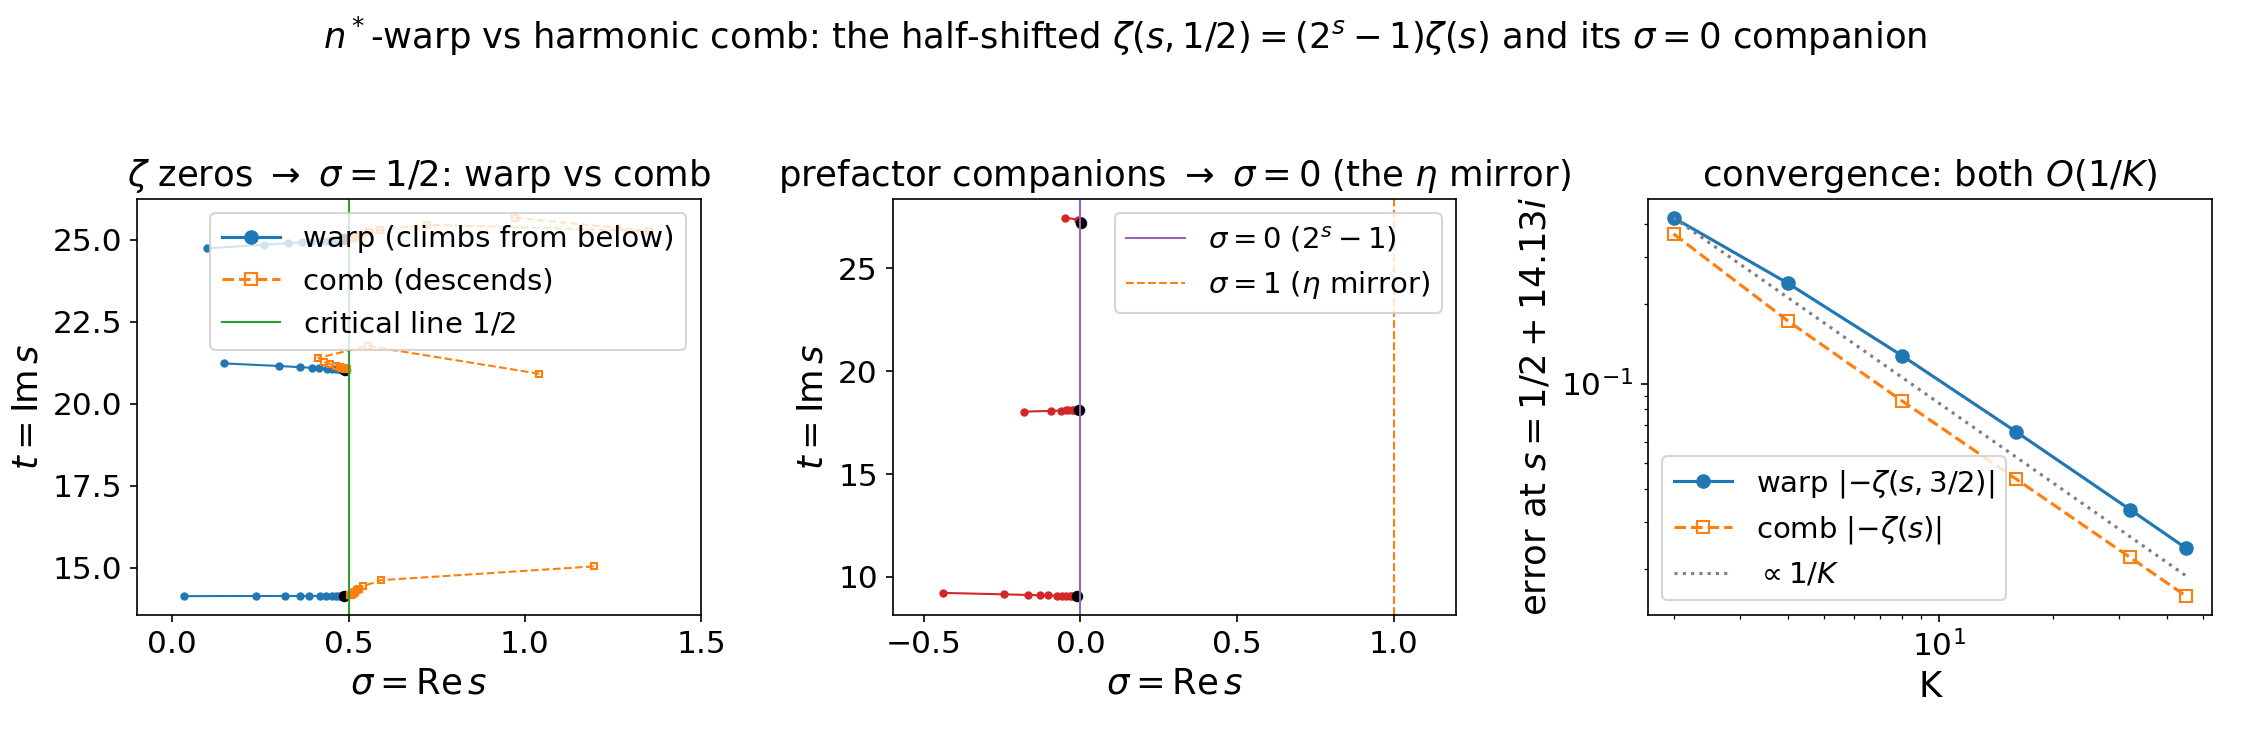
\includegraphics[width=0.92\textwidth]{warp_bridge.png}
  \caption{The nonlinear midpoint warp vs.\ the additive comb. The warp collapses
  each unit cell onto its midpoint, so it targets $\zeta(s,\tfrac12) =
  (2^{s}-1)\zeta(s)$ on the nose: $\zeta$'s zeros climb onto $\sigma=\tfrac12$
  \emph{from below}, and the $2^{s}-1$ companion migrates onto $\sigma=0$ (the
  functional-equation mirror of $\eta$'s $\sigma=1$ comb). The two routes reach
  the critical line by \emph{opposite} approaches, a contrast the rate law
  (\cref{sec:rate}) explains quantitatively.}
  \label{fig:warp}
\end{figure}

\subsection{The warp coordinate, visualized}

\Cref{fig:warpcoord} pictures the warp itself rather than its zeros. The warp
coordinate $n^\ast(x) = x + \varphi_K(x)$ starts as the linear $x$ at $K=0$ and,
as harmonics are restored, bends into the midpoint staircase $\lfloor
x\rfloor+\tfrac12$, collapsing each unit cell onto its midpoint. The cell
midpoints $m+\tfrac12$ are exact fixed points at every $K$. Because the
underlying sawtooth has a unit jump at each integer, the partial sums carry the
classic ${\sim}9\%$ Gibbs overshoot at the step edges, which narrows but never
vanishes. That never-vanishing Gibbs boundary layer is precisely why the warp's
rate constant is a non-elementary sine-integral rather than the comb's clean
$s/2\pi^2$ (\cref{sec:rate}).

\begin{figure}[t]
  \centering
  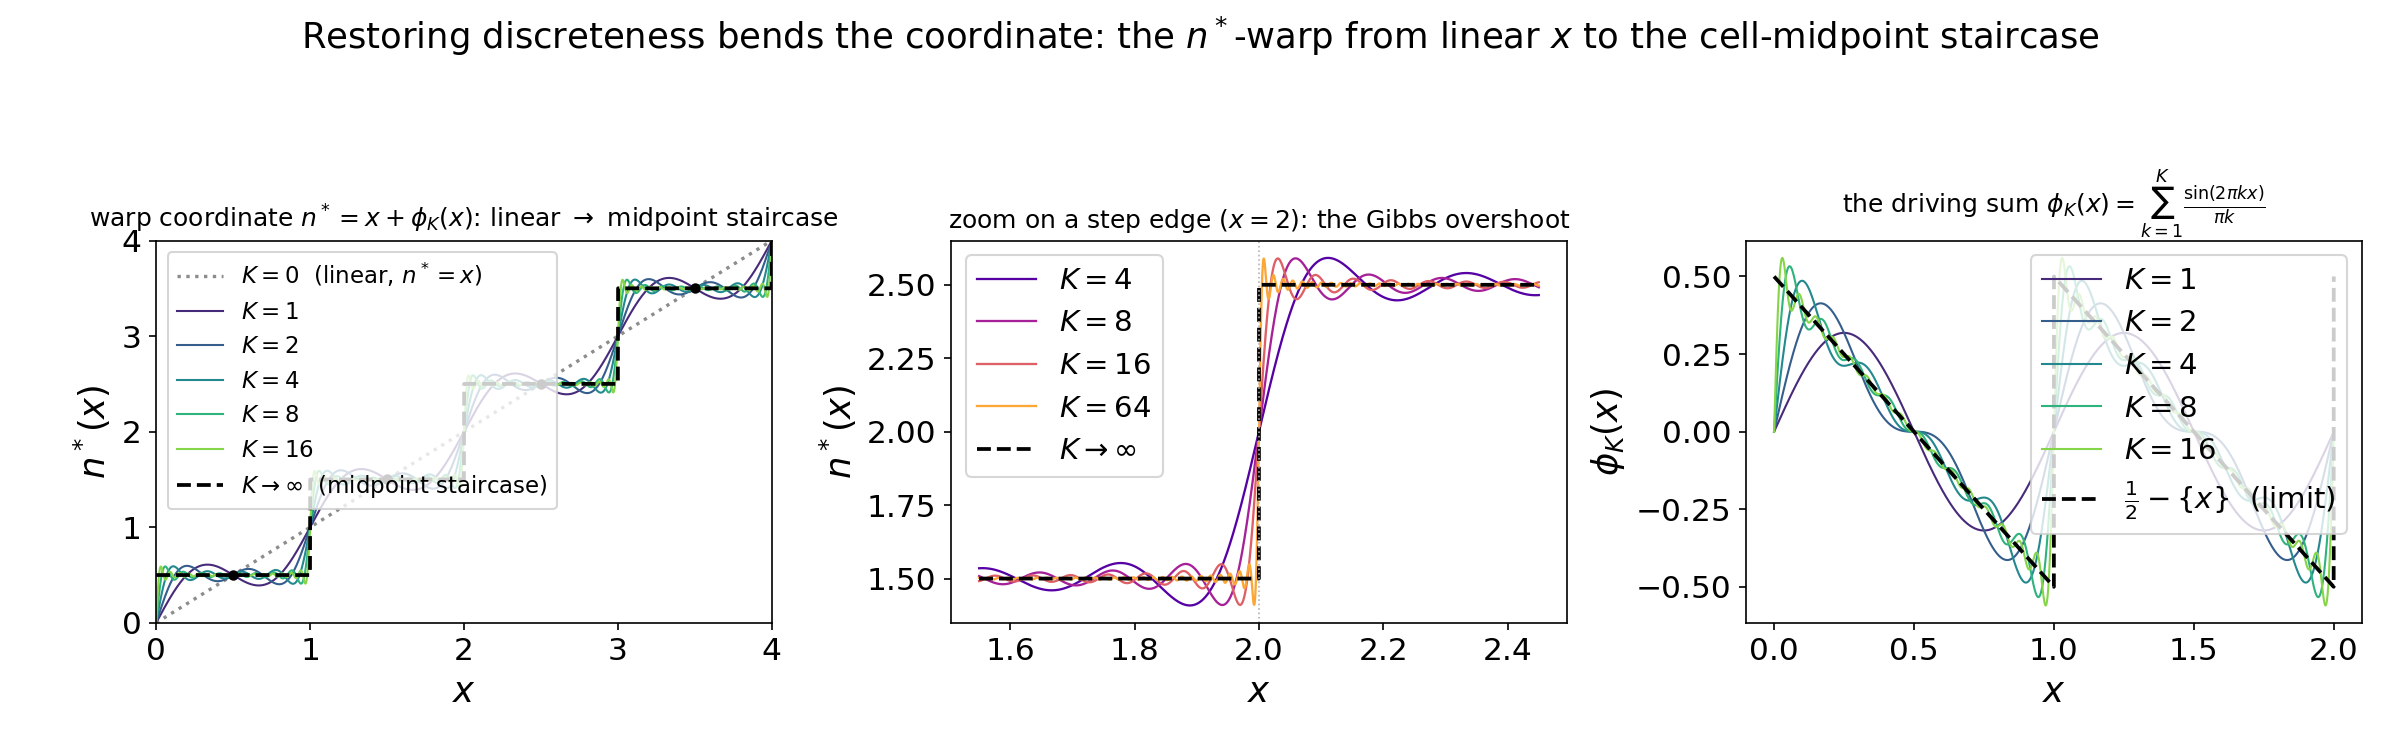
\includegraphics[width=0.92\textwidth]{warp_coordinate.png}
  \caption{The warp coordinate $n^\ast(x)=x+\varphi_K(x)$ bending from the linear
  $x$ ($K=0$) into the midpoint staircase $\lfloor x\rfloor+\tfrac12$ as Fourier
  harmonics are restored. Panel (b): the ${\sim}9\%$ Gibbs overshoot at the step
  edges, which narrows but never vanishes, the source of the warp's
  non-elementary rate constant.}
  \label{fig:warpcoord}
\end{figure}

\subsection{Half-integers vs.\ counting numbers: why $\alpha=\tfrac12$ is the
headline}\label{sec:phasecompare}

Why does the staircase land on the half-integers rather than the counting
numbers? Both are reachable: they are the $\alpha=\tfrac12$ and $\alpha=1$
cases of the general-phase warp (\cref{sec:alpha}), whose cells collapse onto
$\lfloor x\rfloor+\alpha$ via the DC-shifted displacement
$\varphi_K^{(\alpha)}(x) = (\alpha-\tfrac12)+\varphi_K(x)\to\alpha-\{x\}$.
\Cref{fig:phasecompare} puts them side by side. The obstruction to having both is
the constant ($k=0$, DC) Fourier coefficient: the $\alpha=\tfrac12$ displacement
is the \emph{pure} sawtooth $\varphi_K$ (zero mean), while $\alpha=1$ carries a
constant $+\tfrac12$.

\begin{table}[t]
  \centering
  \begin{tabularx}{\textwidth}{@{}lXXX@{}}
    \toprule
     & steps land on & $K=0$ endpoint & $K\to\infty$ target \\
    \midrule
    $\alpha=\tfrac12$ (midpoint, headline) & half-integers $\tfrac12,\tfrac32,\dots$
      & $x$ (pristine $1/(s-1)$) & $(2^{s}-1)\zeta(s)=\zeta(s,\tfrac12)$ \\
    $\alpha=1$ (integer) & counting numbers $1,2,3,\dots$
      & $x+\tfrac12$ (DC offset on) & $\zeta(s,1)=\zeta(s)$ \\
    \bottomrule
  \end{tabularx}
  \caption{The trade-off: a zero-mean periodic correction added to $x$ can only
  ever reach $\lfloor x\rfloor+\tfrac12$. Landing on the integers \emph{requires}
  the non-trigonometric constant $\tfrac12$, so at $K=0$ one is already at
  $x+\tfrac12$, no longer the bland trig-free $x$. One can have a pure-$x$ start
  \emph{or} integer steps, not both.}
  \label{tab:phasecompare}
\end{table}

\begin{figure}[t]
  \centering
  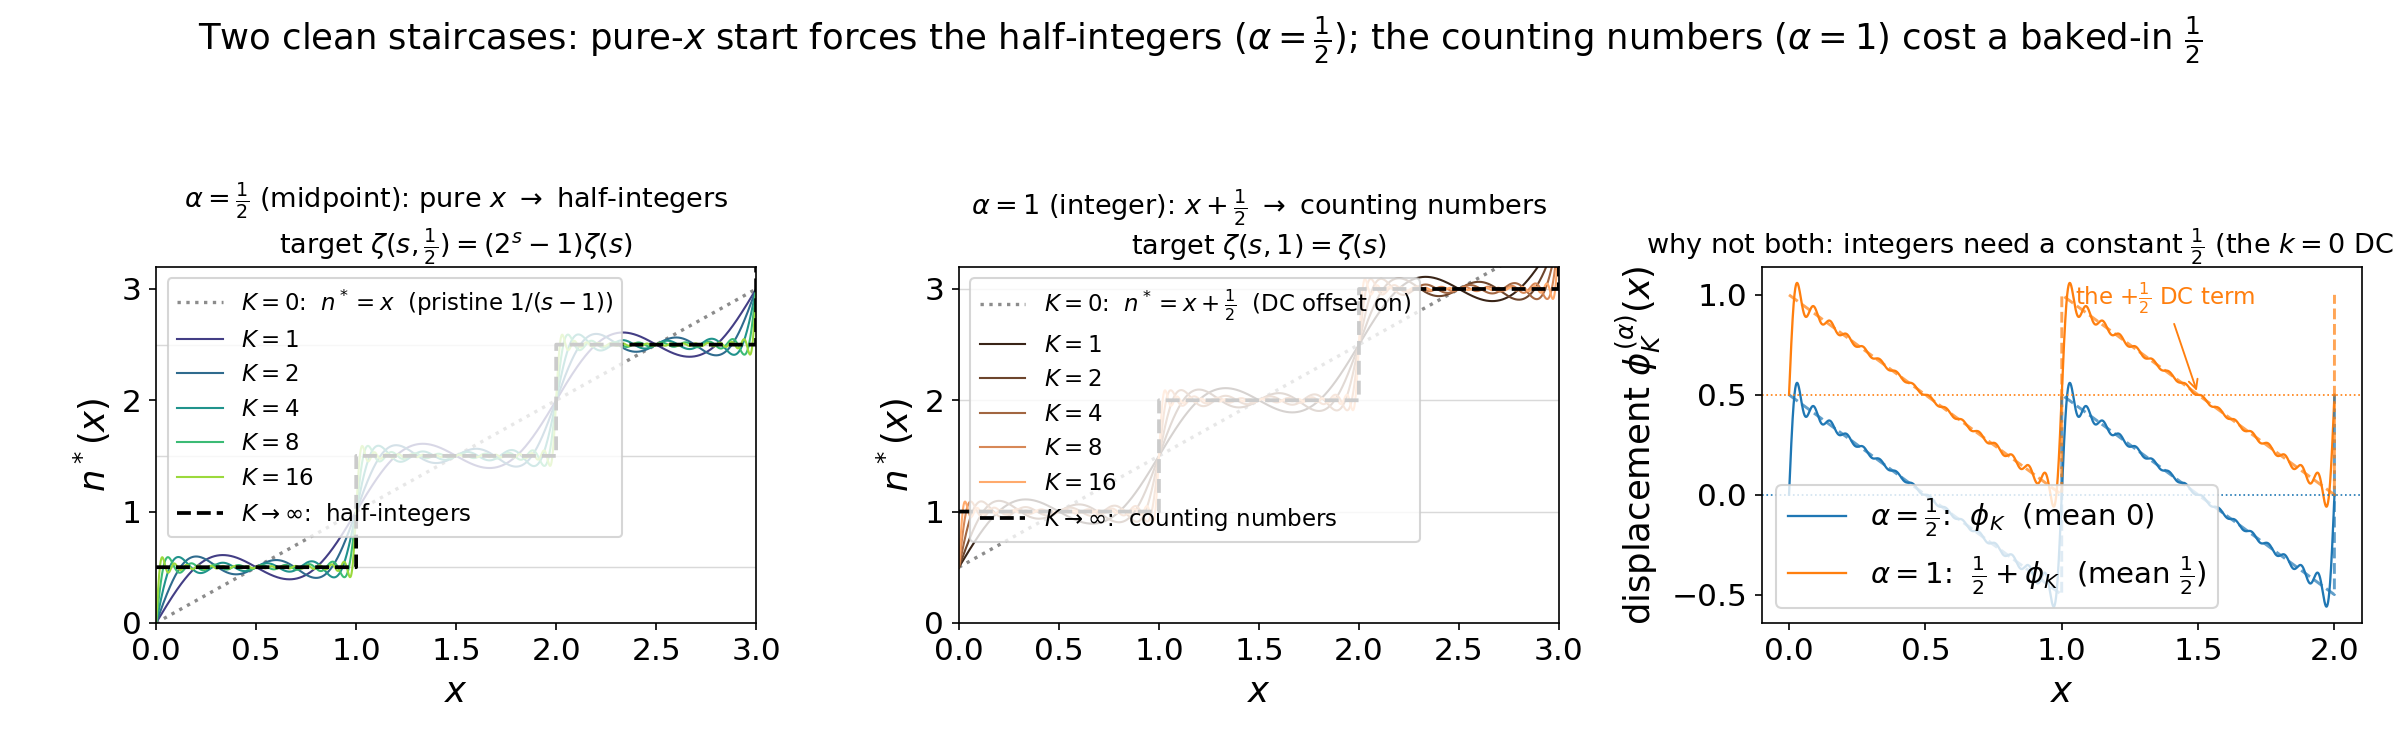
\includegraphics[width=0.92\textwidth]{warp_phase_compare.png}
  \caption{Two clean staircases: $\alpha=\tfrac12$ (half-integers) and $\alpha=1$
  (counting numbers). Panel (c) shows the obstruction: the $\alpha=1$
  displacement carries a constant DC term while $\alpha=\tfrac12$ does not. The
  half-integer midpoint is the \emph{unique} clean staircase reachable from a
  pure-$x$ start by pure trigonometric corrections, which is why it is the
  bridge's headline phase.}
  \label{fig:phasecompare}
\end{figure}

This is why the bridge's headline is $\alpha=\tfrac12$: it is the one phase that
keeps the pristine zeroless endpoint \eqref{eq:bland} \emph{and} lands on a clean
line, and that line is the richer half-shifted $(2^{s}-1)\zeta(s)$, whose
$\sigma=\tfrac12$ zeros are $\zeta$'s own (\cref{sec:legit}) and which also
carries the $\sigma=0$ companion. Choosing $\alpha=1$ recovers plain $\zeta(s)$
and the literal counting numbers, but at the cost of the pristine endpoint
\emph{and} the companion line.

% =====================================================================
\section{The general phase and the $P\cdot L$ dichotomy}\label{sec:alpha}
% =====================================================================

Generalizing the warp to pin cells to an arbitrary phase $n+\alpha$,
$\alpha\in(0,1)$, the completed target is the Hurwitz zeta $\zeta(s,\alpha)$.
Sweeping $\alpha$ and watching where the zeros go exhibits the
Saias--Weingartner $P\cdot L$ dichotomy \citep{SaiasWeingartner2009}: clean
vertical zero strings appear \emph{only} at $\alpha\in\{0,\tfrac12,1\}$, the
phases at which $\zeta(s,\alpha)$ factors as a polynomial in prime powers times a
single Dirichlet $L$-function. (For $\alpha=\tfrac12$ this is
\eqref{eq:halfshift}; in the language of \citealp{SaiasWeingartner2009} the
relevant identity is $(1-2^{-s})\zeta(s) = P(s)\,L(s,\chi_0)$, with $2^{s}$ entire
and nonvanishing.) Every \emph{generic} $\alpha$ gives a Davenport--Heilbronn
scattered set, with zeros off any vertical line and even into $\sigma>1$
\citep{DavenportHeilbronn1936,Cassels1961,SaiasWeingartner2009}; see also the
value-distribution results for algebraic-irrational $\alpha$ in
\citet{SourmelidisSteuding2022}.

\begin{figure}[t]
  \centering
  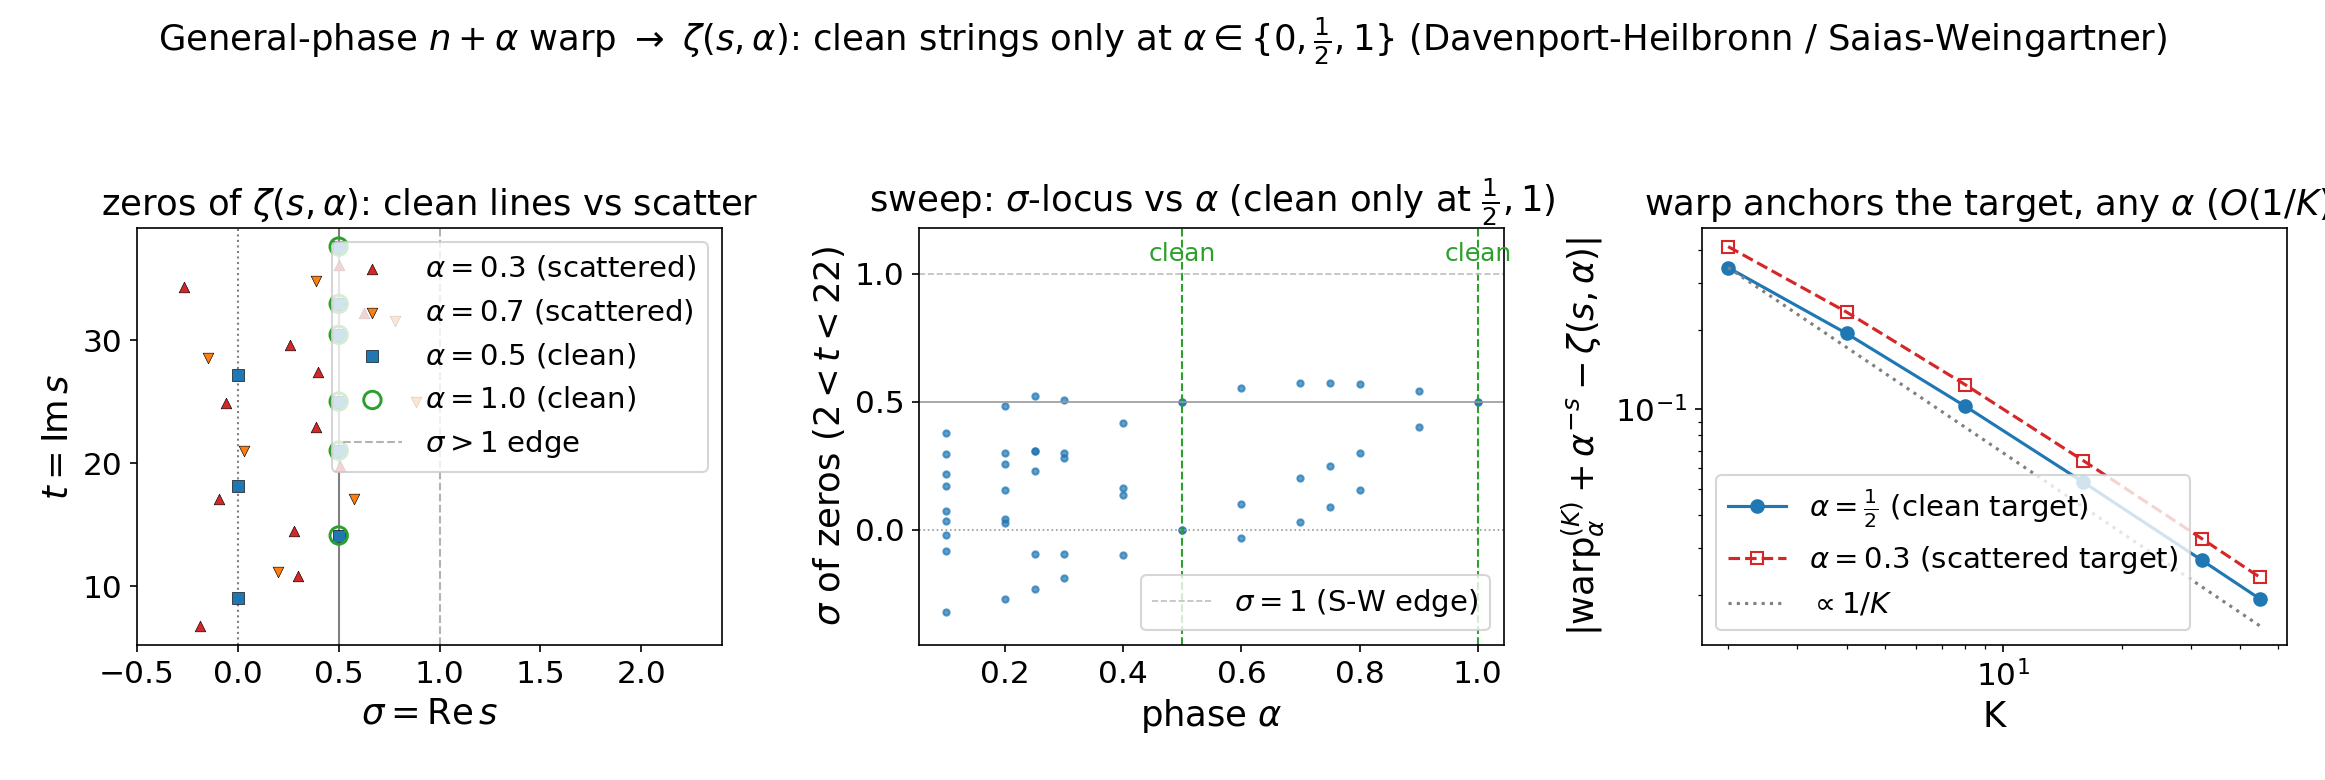
\includegraphics[width=0.92\textwidth]{warp_alpha.png}
  \caption{The general-phase $n+\alpha$ warp onto $\zeta(s,\alpha)$, exhibiting
  the Saias--Weingartner dichotomy: clean vertical strings only at
  $\alpha\in\{0,\tfrac12,1\}$; every generic $\alpha$ is Davenport--Heilbronn
  scattered off-line. This locates the half-shift of \cref{sec:warp} inside a
  one-parameter family and explains why $\tfrac12$ is \emph{special} rather than
  merely chosen.}
  \label{fig:alpha}
\end{figure}

This locates the half-shift of \cref{sec:warp} inside a one-parameter family and
explains why $\tfrac12$ is special rather than merely chosen: it is one of the
three privileged phases. The ``clean lines only at $\{0,\tfrac12,1\}$'' picture
is the load-bearing control that keeps the half-shift route honest.

% =====================================================================
\section{The unified $O(1/K)$ rate law}\label{sec:rate}
% =====================================================================

The synthesis is that one mechanism sits behind every route. All routes truncate
the \emph{same} sawtooth \eqref{eq:sawtooth}, whose retained tail has power
\begin{equation}\label{eq:tail}
  \sum_{k>K}\frac{1}{(\pi k)^2} \sim \frac{1}{\pi^2 K},
\end{equation}
so every route converges as $O(1/K)$. A single zero-displacement law,
\begin{equation}\label{eq:disp}
  s_K - \rho \;\sim\; \frac{a_1(\rho)}{K},
\end{equation}
covers all five zero families (the $\zeta$ comb, the $\eta$ split onto
$\sigma=\tfrac12$ and $\sigma=1$, and the warp's $\sigma=\tfrac12$ and $\sigma=0$
families), with a route- and zero-dependent complex displacement constant
$a_1(\rho)$. The structure of $a_1$ carries the qualitative behavior:

\begin{itemize}[leftmargin=1.4em]
\item \textbf{Approach side $=\operatorname{sign}(\Re a_1)$.} The real part of
  $a_1$ fixes which side the zero approaches its line from, which is why the comb
  descends (and can overshoot) while the warp climbs from below and never
  overshoots; overshoot occurs precisely when $\Re a_1<0$.
\item \textbf{Birth-$K$ law.} The first $K$ that resolves a given zero to
  tolerance $\varepsilon$ is $K_{\mathrm{catch}} = |\Re a_1|/\varepsilon$. This
  ties the birth order of zeros to the Montgomery $a$-values $1/|\zeta'(\rho)|$.
\item \textbf{Vertical migration $=$ Gram's law.} The imaginary part $\Im a_1$
  gives the vertical (along-$t$) migration. Its sign tracks Gram's law
  numerically: it first flips at the classical Gram-law failures
  (zeros $n=127,136,196$).
\end{itemize}

\begin{figure}[t]
  \centering
  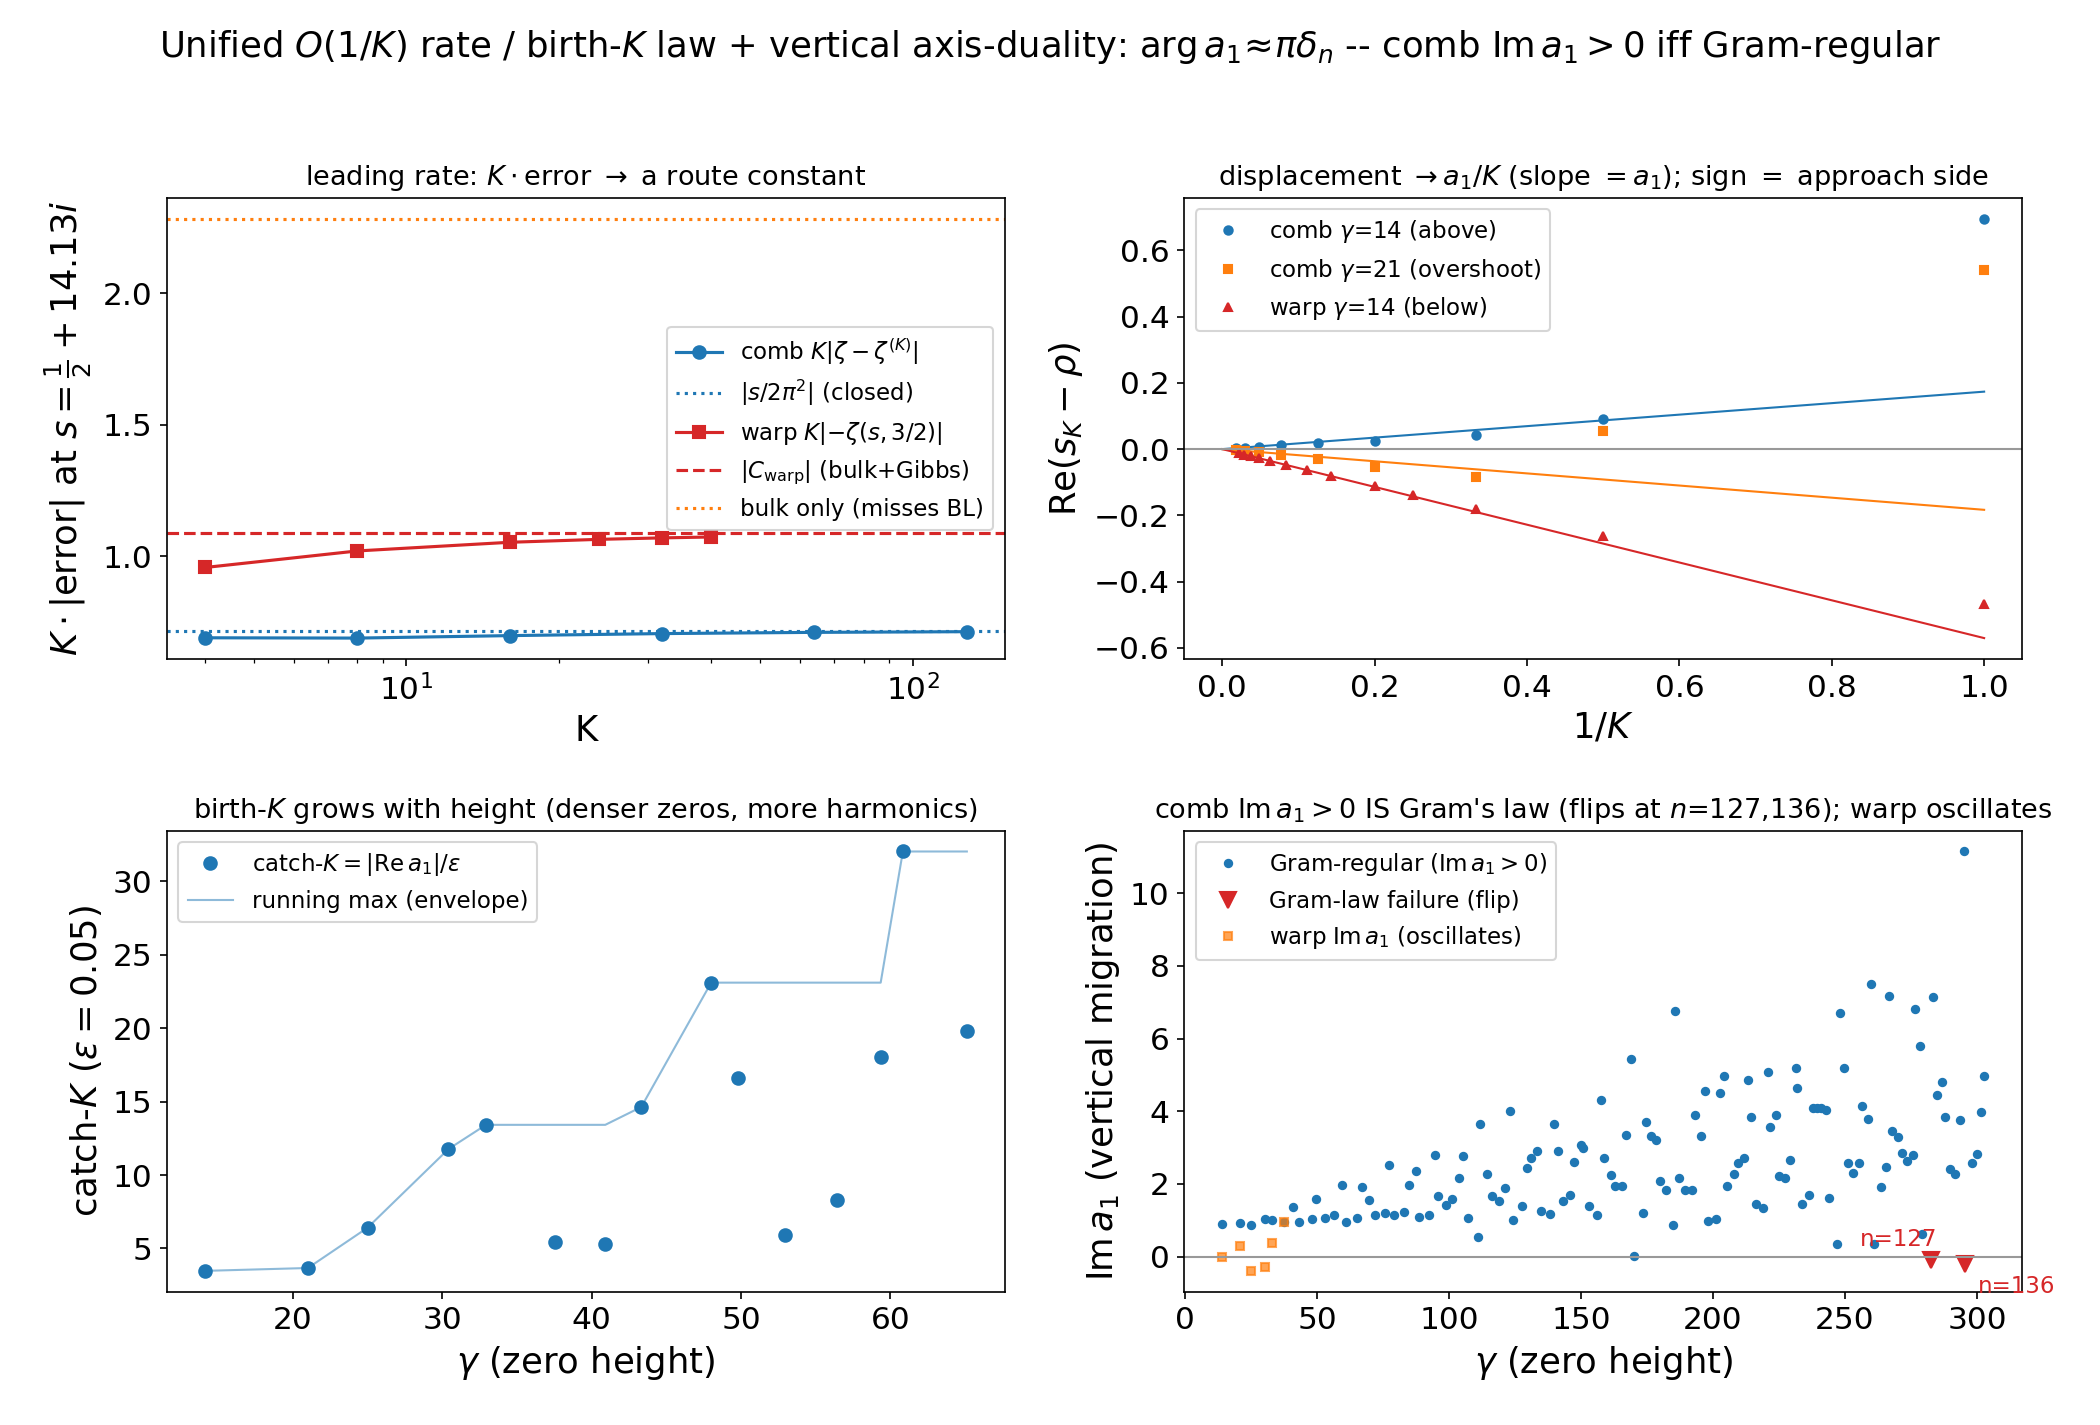
\includegraphics[width=0.92\textwidth]{rate_law.png}
  \caption{The unified $O(1/K)$ rate / birth-$K$ law and the vertical
  axis-duality. All routes truncate the same sawtooth, so all converge as
  $O(1/K)$ \eqref{eq:tail}; the displacement constant $a_1(\rho)$ of
  \eqref{eq:disp} controls approach side ($\operatorname{sign}\Re a_1$),
  birth order ($K_{\mathrm{catch}}=|\Re a_1|/\varepsilon$), and the vertical
  migration ($\Im a_1$), whose sign tracks Gram's law.}
  \label{fig:rate}
\end{figure}

\begin{figure}[t]
  \centering
  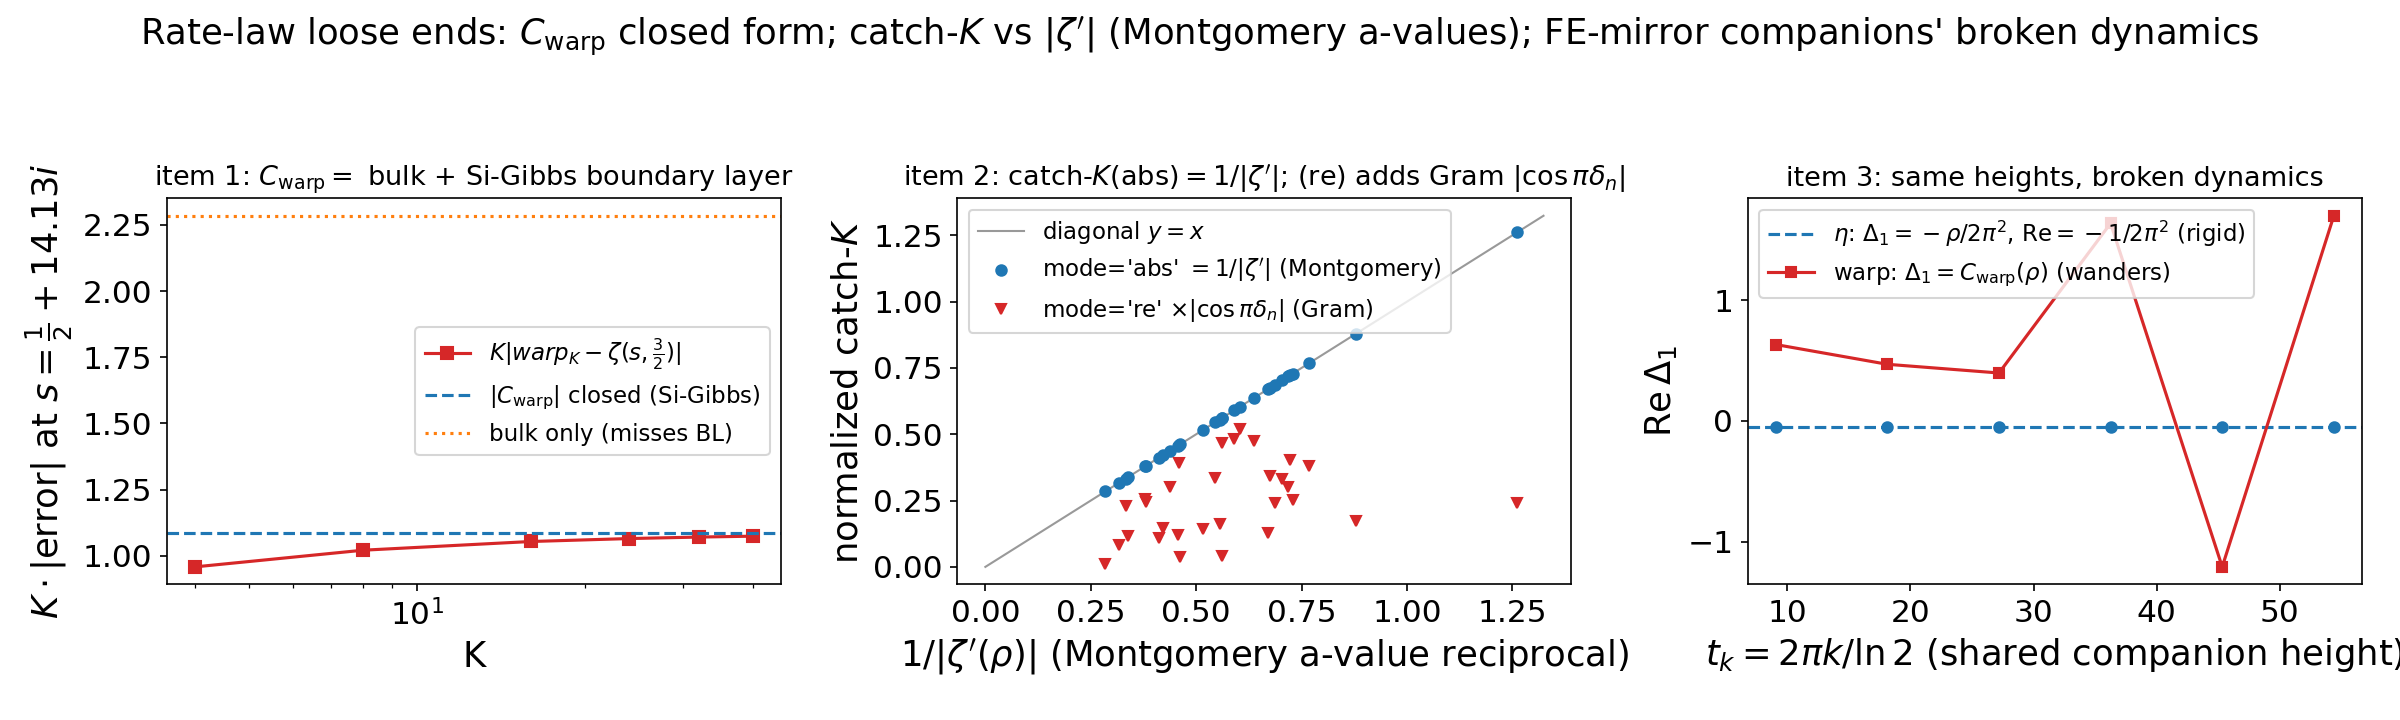
\includegraphics[width=0.92\textwidth]{rate_law_loose_ends.png}
  \caption{Three loose ends of the rate law: (i) a closed form for the warp
  constant $C_{\mathrm{warp}}$ as a Gibbs boundary-layer (sine-integral)
  integral; (ii) the tie of the birth threshold $K_{\mathrm{catch}}$ to the
  Montgomery $a$-values $1/|\zeta'(\rho)|$; and (iii) the fact that the
  $\sigma=1$/$\sigma=0$ companions share heights but \emph{not} migration
  dynamics.}
  \label{fig:rateloose}
\end{figure}

This is where the package stops being several separate demonstrations and becomes
one law: a single rate constant and displacement coefficient, route by route,
plus a Gram's-law coupling on the vertical axis. It is the synthesis around which
the whole study is organized.

% =====================================================================
\section{The two-component $\eta$ spectrum}\label{sec:two}
% =====================================================================

Projected onto the $t$-axis, the $\eta$ zero set is a \emph{rigid crystalline
comb} ($\sigma=1$ teeth at $t=2\pi k/\ln 2$, perfectly periodic) \emph{superposed}
with a \emph{GUE-random sequence} (the $\sigma=\tfrac12$ $\zeta$ zeros)
\citep{Montgomery1973,Odlyzko1987}. \Cref{fig:two} applies three lenses:

\begin{enumerate}[leftmargin=1.6em]
\item \textbf{One-point packing.} There are $\log_2(t/2\pi)$ zeros per comb gap,
  equidistributed.
\item \textbf{Two-point number variance.} In the smooth bulk both lenses say the
  components behave as an \emph{independent superposition}.
\item \textbf{Resonance at the comb frequency.} The third lens shows they are
  \emph{not} independent. The comb teeth sit at the $p=2$ prime-power frequencies
  $m\ln 2$, and by the explicit formula the $\zeta$-zero density carries an
  oscillation at every prime-power frequency, so probing the zeros at the comb
  frequency \emph{resonates}: the measured $\langle\cos(m\gamma\ln 2)\rangle$
  matches the $p=2^m$ explicit-formula coefficient to ${\sim}4$ digits, with a
  negative sign (the comb teeth sit at density \emph{minima}).
\end{enumerate}

The $\sigma=1$ comb is, in this sense, the ``$p=2$ ghost'' of the zeros' own
prime structure.

\begin{figure}[t]
  \centering
  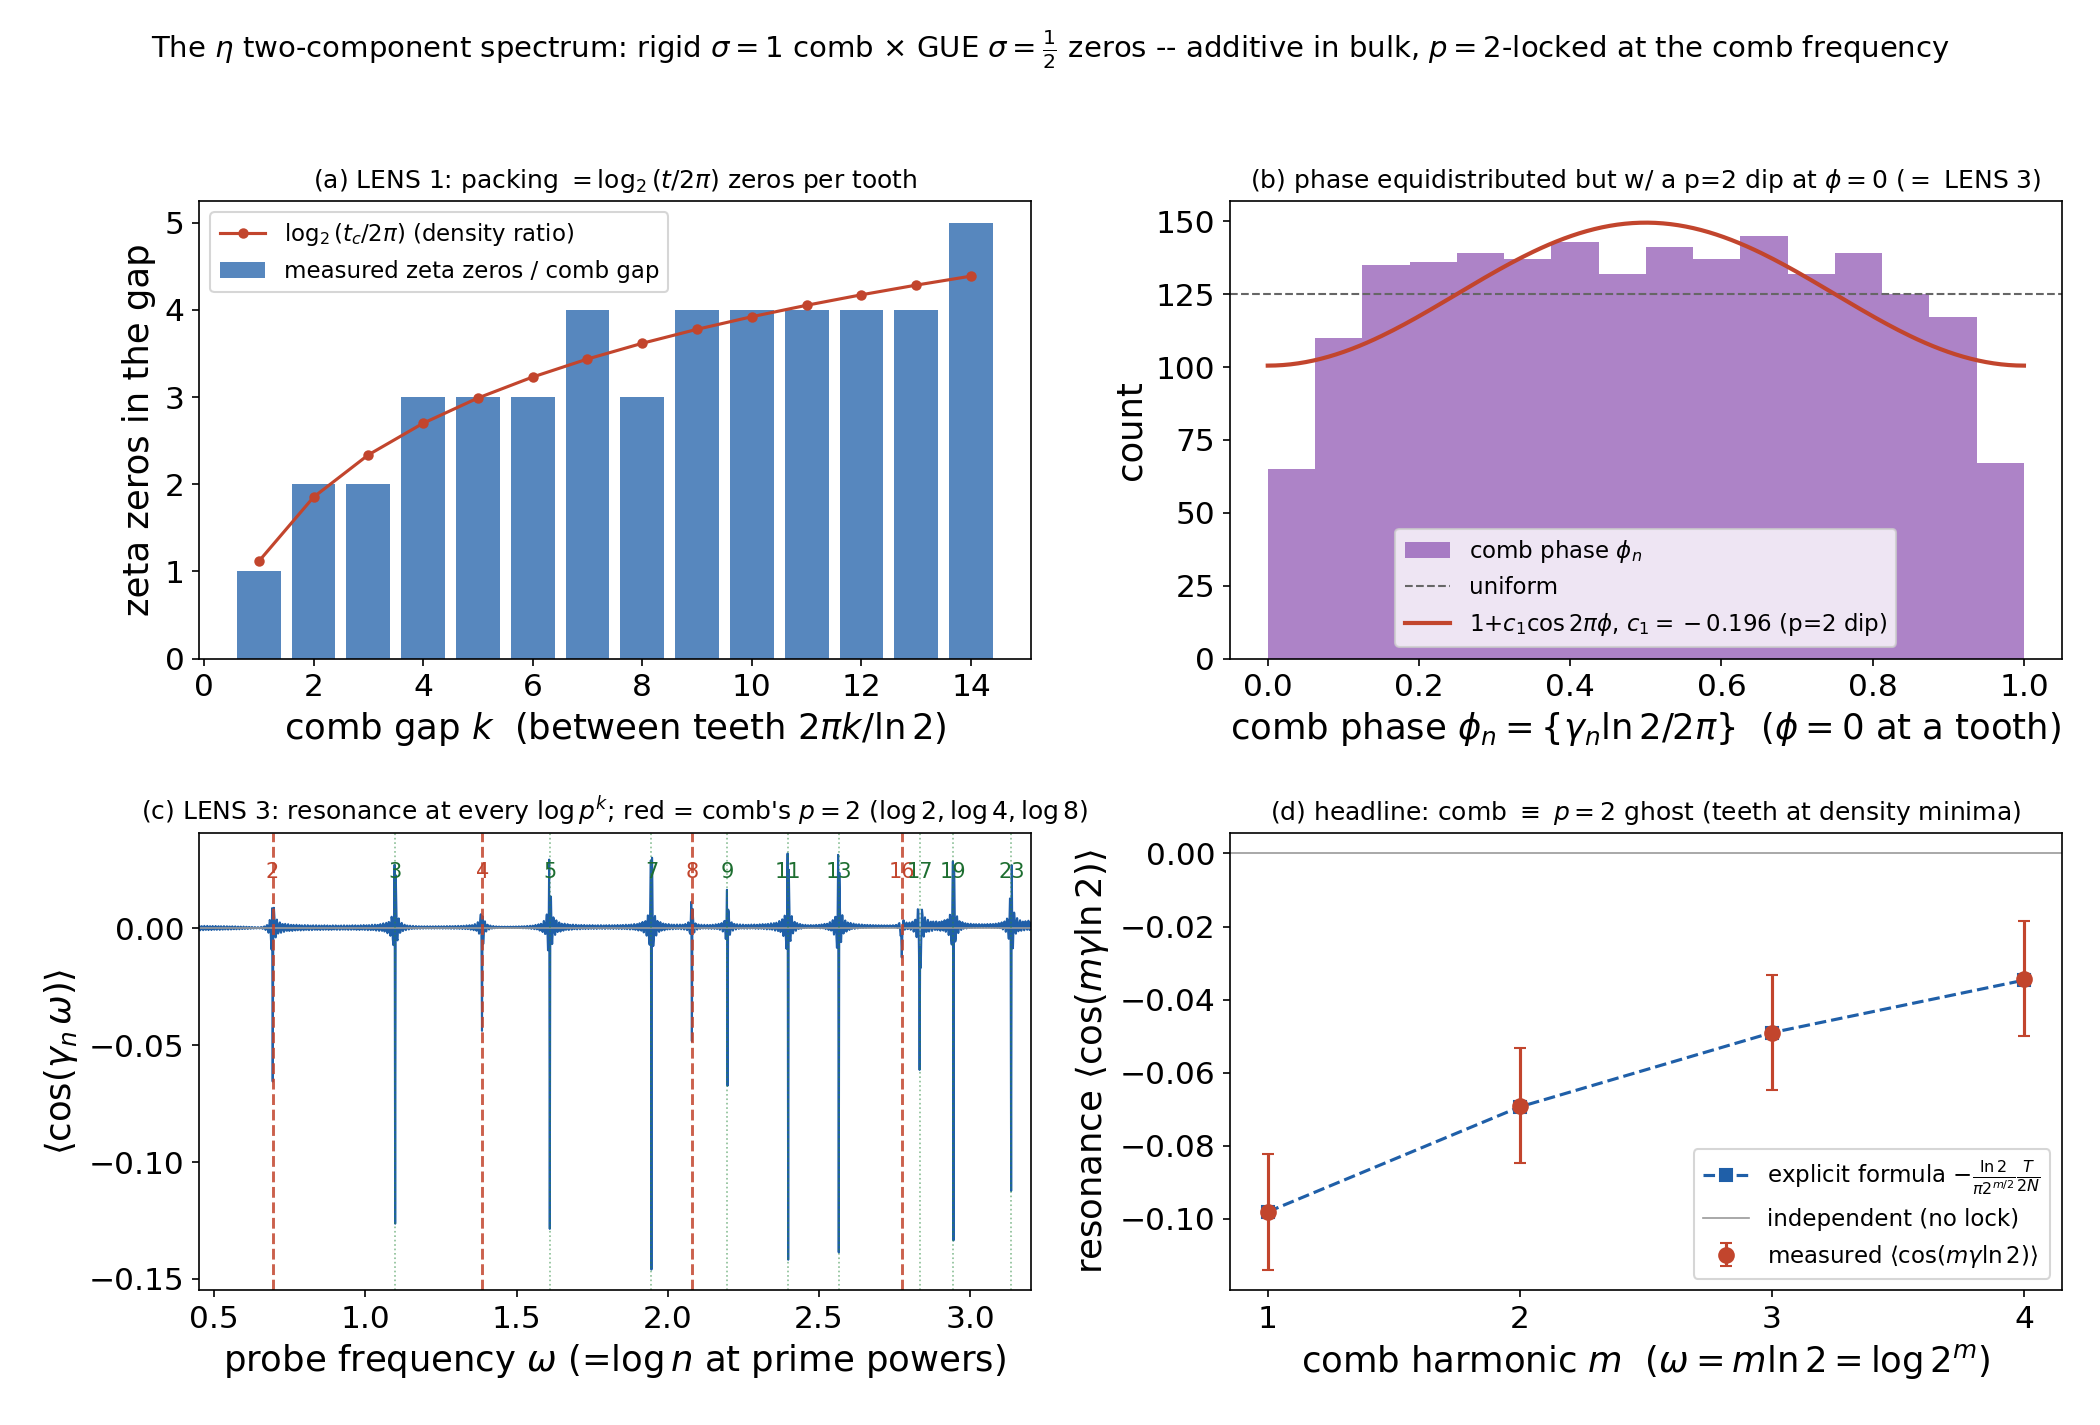
\includegraphics[width=0.92\textwidth]{eta_two_component.png}
  \caption{The $\eta$ zeros as a two-component ``crystal $\times$ GUE'' spectrum:
  a rigid $\sigma=1$ comb at $t=2\pi k/\ln 2$ superposed on the
  $\sigma=\tfrac12$ GUE $\zeta$-zeros. The comb frequencies $m\ln 2$ are the
  $p=2$ prime-power frequencies; probing the zeros there resonates with the
  explicit-formula coefficient (the ``$p=2$ ghost'').}
  \label{fig:two}
\end{figure}

\begin{remark}[Honest caveat]\label{rmk:caveat}
The appearance of $\ln 2$ in the zeros' number variance is \emph{not} new. Berry
\citep{Berry1988}, made rigorous by Lugar, Milinovich and Quesada-Herrera
\citep{LugarMilinovichQuesadaHerrera2022}, already places prime-power
log-frequencies in the zeta-zero number variance in a regime where the GUE
prediction fails, and $\ln 2$ is the \emph{single lowest} such frequency (note
$\ln 3 < \ln 4 = 2\ln 2$, so $\ln 2$ is lowest but the band is not simply the
multiples of $\ln 2$). What is ours here is only the comb\,$\uplus$\,GUE
\emph{superposition} model, the \emph{single-prime isolation} ($p=2$), and the
\emph{eta tie-in} (relating the $\sigma=1$ eta comb to that lattice), not the
$\ln 2$ frequency itself. See \cref{sec:prior}.
\end{remark}

% =====================================================================
\section{Relation to prior work}\label{sec:prior}
% =====================================================================

The endpoints and most ingredients of this study are classical; we cite them
rather than claim them. We have made two adversarial passes through the
literature, and we foreground the two closest prior-art results explicitly so a
reader can locate our residual contribution precisely.

\subsection{Cite, do not claim}
\begin{itemize}[leftmargin=1.4em]
\item The half-shift $(2^{s}-1)\zeta(s)=\zeta(s,\tfrac12)$, its $\sigma=0$
  companion at $t=2\pi k/\ln 2$, and the migration of Hurwitz-type zeros onto
  $\sigma=\tfrac12$ as a parameter varies: \citet{Gonek1981,GarunkstisSteuding2007};
  see also \citet{GarunkstisTamosiunas2013} for the periodic-Hurwitz
  Riemann--von Mangoldt counting law.
\item The $\alpha\in\{0,\tfrac12,1\}$ ``clean lines only'' dichotomy:
  \citet{SaiasWeingartner2009}; generic off-line $\zeta(s,\alpha)$ zeros:
  \citet{DavenportHeilbronn1936,Cassels1961}.
\item The $\sigma=1$ eta comb at $t=2\pi k/\ln 2$: \citet{Sondow2003};
  tabulated by \citet{BeliakovMatiyasevich2015}; \citealp[\S25.2.3]{DLMF}.
\item The closest ``knob'' cousins use partial-sum \emph{length} $N$ rather than
  the harmonic count $K$, and none start from a zeroless endpoint:
  \citet{GonekLedoan2010,GonekMontgomery2013}; see also
  \citet{PlattTrudgian2016}. Zeros of combinations of Euler products for
  $\sigma>1$: \citet{BookerThorne2014,Righetti2016}. A numerical study of the
  off-line zeros of the Davenport--Heilbronn counterexample (by a
  deform-and-track homotopy): \citet{BalanzarioSanchezOrtiz2007}.
\end{itemize}

\subsection{The deflator to foreground (the $p=2$ ghost)}
As stated in \cref{rmk:caveat}, the strongest prior art for the two-component
reading is \citet{Berry1988}, proved by
\citet{LugarMilinovichQuesadaHerrera2022}: the number variance
$\Sigma^2(L)$ of the Riemann zeros has a prime-controlled regime in which the GUE
prediction explicitly fails, governed by a von Mangoldt cosine sum at frequencies
$\ln n$ whose single smallest is $\ln 2$. That work treats the \emph{single}
zeta-zero spectrum; it does not treat the Dirichlet-$\eta$ / partial-sum zeros,
does not build the comb\,$\uplus$\,GUE two-spectrum superposition statistics, does
not isolate a single prime, and does not tie the $\sigma=1$ eta comb at
$t=2\pi k/\ln 2$ to the $p=2$ lattice via the explicit formula. Those four are
the surviving contribution of \cref{sec:two}. Related ``quasicrystal''
readings of the zeros (the zero-spacing distributions of differenced
$L$-functions \citep{Lagarias2006}, and prime-power Bragg peaks in the zeros'
structure factor \citep{MadisonMadisonKozyrev2023,Shaughnessy2024}) supply the
``crystal'' half as a single spectrum but not the superposition model;
\citet{MoranLedezma2023} treats the explicit formula as Bohr-space spectral
measures (a value-distribution statement, not a zero-statistics one).

\subsection{Contrast with the de Bruijn--Newman heat flow}
Our deformation should not be confused with the de Bruijn--Newman heat flow. In
that picture the family $H_t = \eu^{t\Delta}H_0$ is, for \emph{every} value of the
flow parameter $t$, an entire function of order one carrying the full infinite
complement of $\xi$-type zeros at Weyl density; the backward heat flow merely
transports these already-existing zeros (by a Calogero--Moser-type ODE)
onto or off the real axis, and the de Bruijn--Newman constant $\Lambda$ (now known
to satisfy $0\le\Lambda\le 0.22$, with RH $\Longleftrightarrow\Lambda=0$ after
\citealp{RodgersTao2020,Polymath2019DBN}) marks the threshold at which an existing
configuration has become entirely real. No zeros are created or destroyed; the
question is purely \emph{when} a fixed-cardinality configuration becomes all-real.
By contrast, our harmonic-count knob $K$ interpolates from a genuinely zeroless
endpoint (the bare continuous integral \eqref{eq:bland}, which has no
non-trivial zeros at all) to the full Dirichlet series, and the non-trivial
zeros are \emph{born} as $K$ increases and then migrate to the critical line.
Ours is a creation-and-migration mechanism from a zeroless endpoint, not a
real-ification of a pre-existing infinite zero set.

\subsection{Contrast with Taylor-section and resummation routes}
Our rate is algebraic, $O(1/K)$ \eqref{eq:tail}. This distinguishes the
construction from the Taylor sections of $\xi$, whose zeros converge
\emph{super-exponentially} \citep{JenkinsMcLaughlin2016}, and from the
Borel/resurgent resummation of the \emph{entire} Euler--Maclaurin remainder
\citep{CostinGaroufalidis2008}, which retains no truncation parameter and births
no zeros. The shared sawtooth tail \eqref{eq:tail} is what makes \emph{our}
family uniformly $O(1/K)$ across all routes.

% =====================================================================
\section{Reproducibility}\label{sec:repro}
% =====================================================================

Every figure in this paper is produced by a driver of the same name in the
accompanying repository, and every driver self-validates its identities to full
precision before it plots, so each figure doubles as a numerical certificate. The
nine figures are regenerated together by a single command:
\begin{quote}
\texttt{python repro.py}\quad(regenerates all figures);\qquad
\texttt{pytest}\quad(fast self-checks; \texttt{pytest -m slow} for the
high-precision suite).
\end{quote}
The drivers are pure \texttt{mpmath} except \texttt{eta\_two\_component.py}, which
additionally reads a cached table of Riemann zeros. The code targets Python~3.9
and is released under the MIT license. Full setup instructions, a
figure-by-figure walkthrough (\texttt{RESULTS.md}), and the annotated
bibliography accompany the source at
\url{https://github.com/bradleypmartin/dirichlet-bridge}.

% =====================================================================
\section*{Acknowledgments}
% =====================================================================
\addcontentsline{toc}{section}{Acknowledgments}
This study was extracted as a self-contained arc from a larger research project.
The novelty framing above rests on two adversarial literature passes; the author
thanks the reviewers and tools that contributed to that vetting. Any errors of
attribution are the author's own.

% =====================================================================
\bibliographystyle{plainnat}
\bibliography{references}

\end{document}
